\chapter{Resultados Parciais}\label{chp:resultados}

Este capítulo apresenta os resultados dos experimentos obtidos até o exame da qualificação. Os experimentos envolvem os algoritmos Método de Katakis (com Ganho de Informação) e o \textit{Online Feature Selection}.

\section{Apresentação e discussão dos resultados}

As Tabelas~\ref{tab:acc_winsize1} e ~\ref{tab:acc_winsize2} apresentam os resultados de acurácia final obtidos nos experimentos realizados, por método, janela de processamento e quantidade de atributos selecionados nas bases de dados reais e artificiais, respectivamente. 

As figuras~\ref{fig:spam_data}, \ref{fig:mailing_list}, \ref{fig:incremental_drift}, \ref{fig:gradual_drift}, \ref{fig:sudden_drift} e \ref{fig:recurrent_drift} apresentam os gráficos de acurácia sequencial (em \%), tempo de resposta (em segundos) e uso de memória RAM (em RAM-horas) por quantidade de fluxos processados por método de seleção de atributos, considerando $winSize=1$, nos conjuntos de dados selecionados.


\begin{table}[!htb]
\centering
\caption[Acurácia final (em \%) por método, janela e quantidade de atributos selecionados das bases reais]{Acurácia final (em \%) por método, janela e quantidade de atributos selecionados das bases reais. O melhor resultado de cada conjunto de dados é destacado em negrito. Nenhuma seleção é realizada na coluna Naïve Bayes}
\label{tab:acc_winsize1}
  \begin{tabular}{lSSSSSSSSS}
    \toprule
    \multirow{2}{*}{} &
      \multicolumn{1}{c}{NB (\%) } &
       \multicolumn{1}{c}{Janela} &
      \multicolumn{3}{c}{MK (\%)} &  
      \multicolumn{3}{c}{OFS (\%)} \\ 
      \cmidrule(lr){4-6}
      \cmidrule(lr){7-9}
      & & & {4} & {10} & {100} & {4} & {10} & {100} \\
      \midrule
      \multirow{4}{*}{spam\_data} & \multirow{4}{*}{74.57} & 1 & 85.81 & \textbf{88.73} & 88.56 & 76.16 & 77.73 & 76.56 \\
     & & 10 & 81.85 & \textbf{83.10} & 82.92 & 75.81 & 77.97 & 76.29\\
     & & 100 & 85.67 & 85.23 & \textbf{86.16} & 76.11 & 77.58 & 73.73\\
    & & 1000 & \textbf{85.73} & 81.50 & 83.22 & 76.03 & 77.37 & 76.31\\
     \multirow{4}{*}{mailing\_list} & \multirow{4}{*}{\textbf{84.60}} & 1 & 60.23 & 66.31 & 80.79 & 53.30 & 53.76 & 56.92 \\
     & & 10 & 60.29 & 70.62 & 78.65 & 58.55 & 59.77 & 64.93\\
     & & 100 & 50.29 & 69.46 & 78.21 & 54.13 & 54.82 & 57.99\\
    & & 1000 & 60.92 & 67.67 & 75.46 & 53.66 & 54.63 & 57.22\\
    \bottomrule
  \end{tabular}
\end{table}

\clearpage

\begin{table}[!ht]
\centering
\caption[Acurácia final (em \%) por método, janela e quantidade de atributos selecionados das bases artificiais]{Acurácia final (em \%) por método, janela e quantidade de atributos selecionados das bases artificiais. O melhor resultado de cada conjunto de dados é destacado em negrito. Nenhuma seleção é realizada na coluna Naïve Bayes}
\label{tab:acc_winsize2}
%[Andre] Deixei todas as colunas centralizadas, exceto a primeira.
\begin{tabular}{lcccc}
    \toprule
   \multirow{2}{*}{} &
      \multicolumn{1}{c}{NB (\%) } &
       \multicolumn{1}{c}{Janela} &
      \multicolumn{1}{c}{MK (\%)} &  
      \multicolumn{1}{c}{OFS (\%)} \\ 
		\midrule
 \multirow{4}{*}{incremental\_drift} & \multirow{4}{*}{\textbf{77.60}} & 1 & 71.60 & 76.93 \\ 
     & & 10 & 71.63 & 77.04 \\
     & & 100 & 71.83 & 77.04\\
    & & 1000 & 71.90 & 76.92\\ 
     \multirow{4}{*}{gradual\_drift} & \multirow{4}{*}{\textbf{92.91}} & 1 & 92.72 & 92.87 \\
    & & 10 & 92.76 & 92.81 \\
     & & 100 & 92.59 & 92.86 \\
    & & 1000 & 92.60 & 92.87\\
    \multirow{4}{*}{sudden\_drift} & \multirow{4}{*}{73.38} & 1 & 77.89 & \textbf{78.11} \\
     & & 10 & 77.90 & \textbf{78.31}\\
     & & 100 & 77.80 & \textbf{78.02}\\
    & & 1000 & 71.00 & \textbf{78.10}\\
    \multirow{4}{*}{recurrent\_drift} & \multirow{4}{*}{\textbf{73.53}} & 1 & 72.18 & 63.69 \\
     & & 10 & 72.10 & 65.34\\
     & & 100 & 72.18 & 64.12\\
    & & 1000 & 67.65& 63.70\\
     \bottomrule
\end{tabular}
\end{table}





\begin{figure}[!htb]
\centering
\begin{subfigure}[b]{0.485\textwidth}
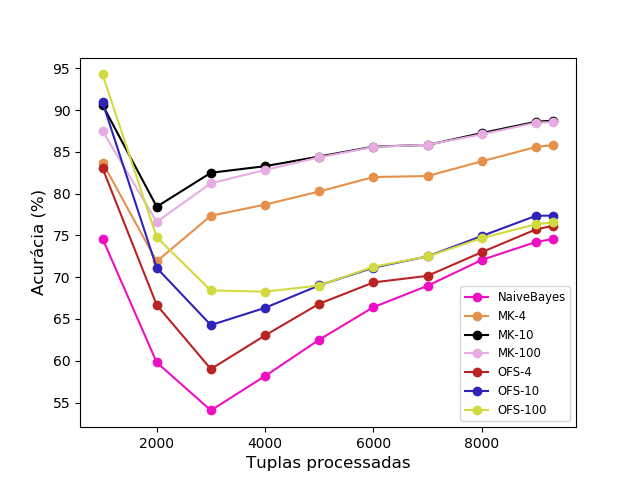
\includegraphics[width=\textwidth]{acc_spam_data.png}
\caption{Acurácia sequencial} \label{fig:spam_data_1a}
\end{subfigure}
%\hspace*{\fill} % separation between the subfigures
\hfill %[Andre] Comentei a linha anterior
\begin{subfigure}[b]{0.485\textwidth}
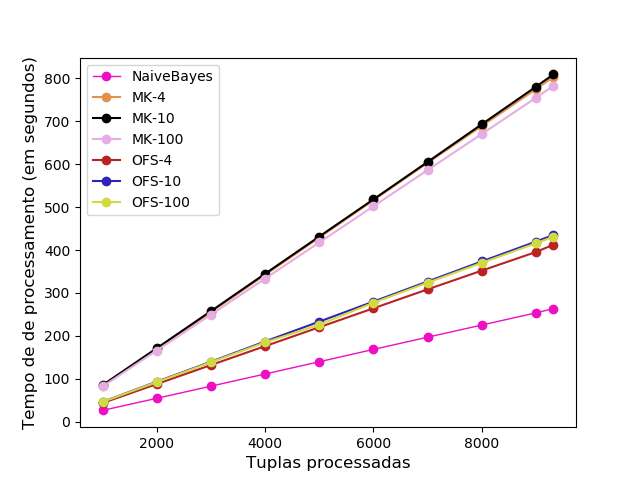
\includegraphics[width=\textwidth]{time_spam_data.png}
\caption{Tempo de resposta} \label{fig:spam_data_1b}
\end{subfigure}
%\hspace*{\fill} % separation between the subfigures
%[Andre] Comentei a linha anterior
\begin{subfigure}[b]{0.5\textwidth}
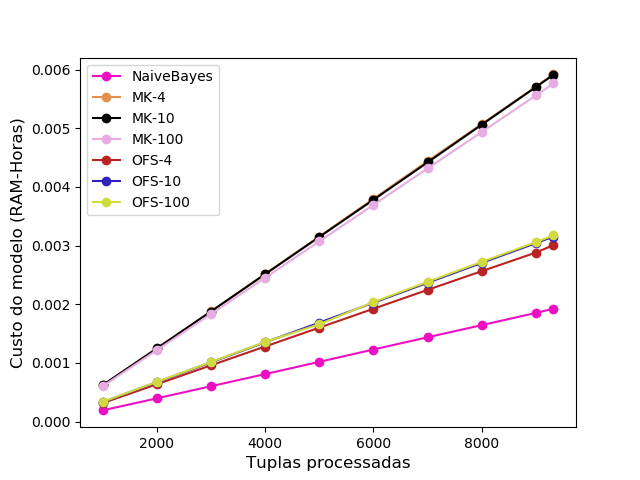
\includegraphics[width=\textwidth]{ram_spam_data.png}
\caption{Uso de memória} \label{fig:spam_data_1c}
\end{subfigure}
\caption[Gráficos de métricas no conjunto de dados \textit{spam\_data}]{Gráficos de métricas no conjunto de dados \textit{spam\_data}.} \label{fig:spam_data}
\end{figure}



\begin{figure}[!htb]
\centering
\begin{subfigure}{0.485\textwidth}
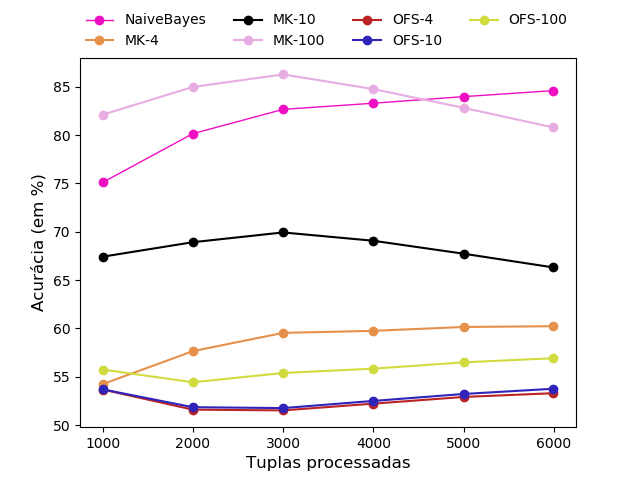
\includegraphics[width=\linewidth]{acc_mailing_list.png}
\caption{Acurácia sequencial} \label{fig:mailing_1a}
\end{subfigure}
%\hspace*{\fill} % separation between the subfigures
\hfill
\begin{subfigure}{0.48\textwidth}
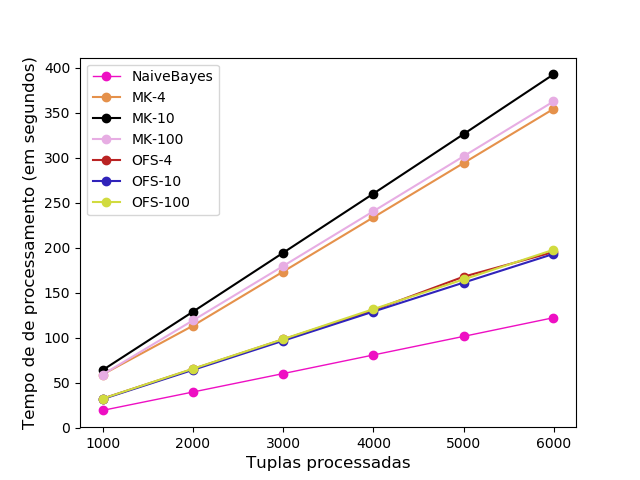
\includegraphics[width=\linewidth]{time_mailing_list.png}
\caption{Tempo de resposta} \label{fig:mailing_1b}
\end{subfigure}
%\hspace*{\fill} % separation between the subfigures
\begin{subfigure}{0.5\textwidth}
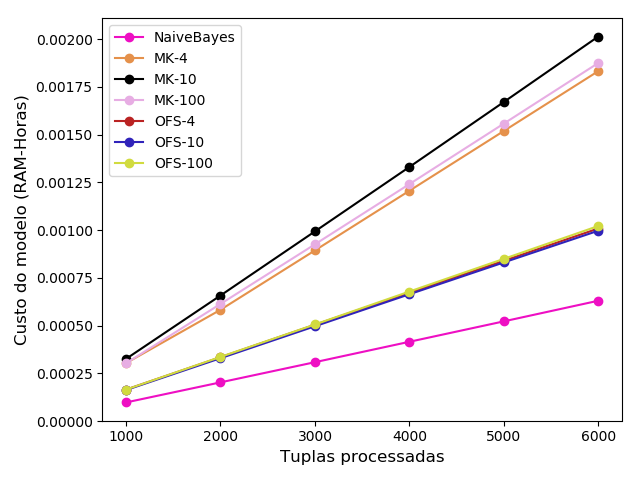
\includegraphics[width=\linewidth]{ram_mailing_list.png}
\caption{Uso de memória} \label{mailing_fig:1c}
\end{subfigure}
\caption[Gráficos de métricas no conjunto de dados \textit{mailing\_list}]{Gráficos de métricas no conjunto de dados \textit{mailing\_list}.} \label{fig:mailing_list}
\end{figure}



\begin{figure}[!htb]
\centering
\begin{subfigure}[t]{0.485\textwidth}
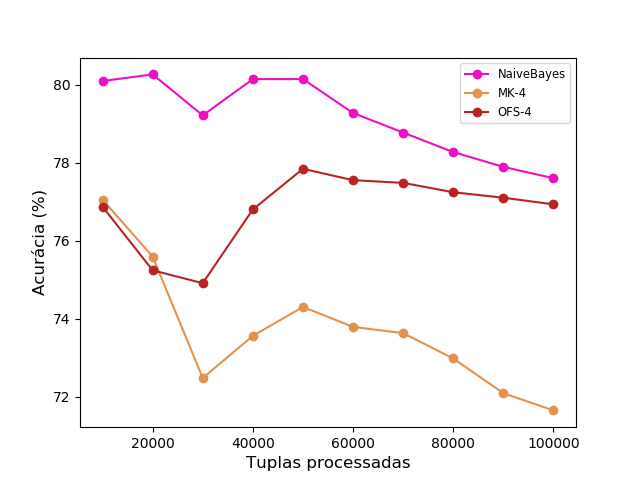
\includegraphics[width=\linewidth]{acc_incremental_drift.png}
\caption{Acurácia sequencial} \label{fig:incremental_1a}
\end{subfigure}
%\hspace*{\fill} % separation between the subfigures
\hfill
\begin{minipage}{\textwidth} 
%[Andre] Adicionei o \begin{minipage} para ajusta o restante das figuras em 4x4
% Note o \end{minipage} no final.
\begin{subfigure}[t]{0.485\textwidth}
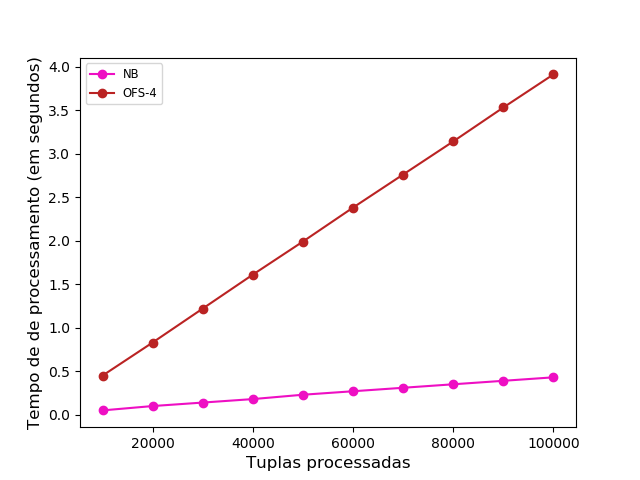
\includegraphics[width=\linewidth]{time_incremental_drift.png}
\caption{Tempo de resposta com Naïve Bayes e OFS-4} \label{fig:incremental_1b}
\end{subfigure}
%\hspace*{\fill} % separation between the subfigures
\hfill
\begin{subfigure}[t]{0.485\textwidth}
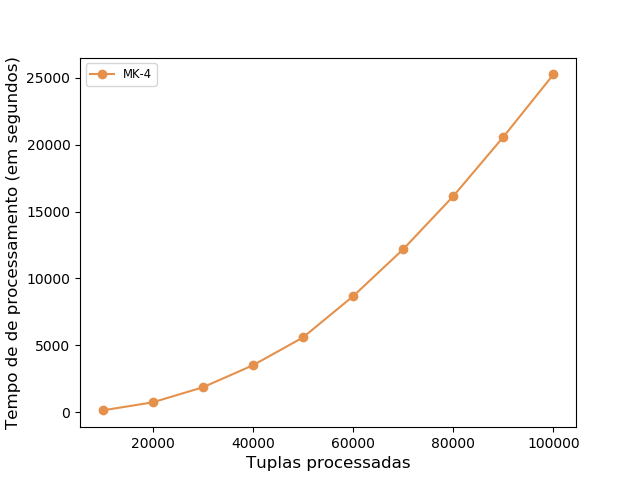
\includegraphics[width=\linewidth]{time_incremental_drift_mk4.png}
\caption{Tempo de resposta para MK-4} \label{fig:incremental_1c}
\end{subfigure}
\hfill
\begin{subfigure}[t]{0.485\textwidth}
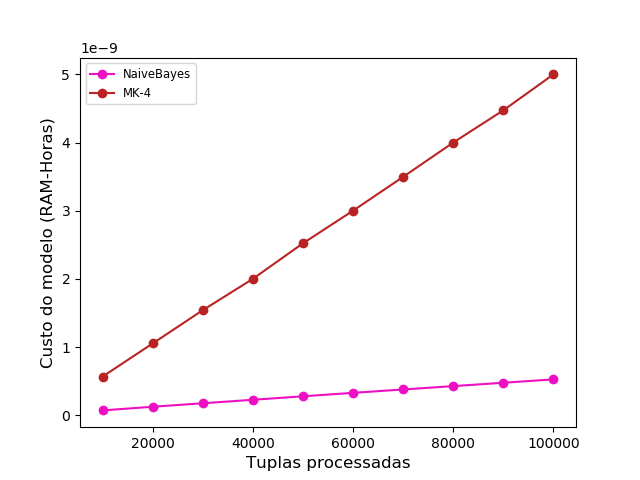
\includegraphics[width=\linewidth]{ram_incremental_drift.png}
\caption{Uso de memória com Naïve Bayes e OFS-4} \label{fig:incremental_1d}
\end{subfigure}
%\hspace*{\fill} % separation between the subfigures
\hfill
\begin{subfigure}[t]{0.485\textwidth}
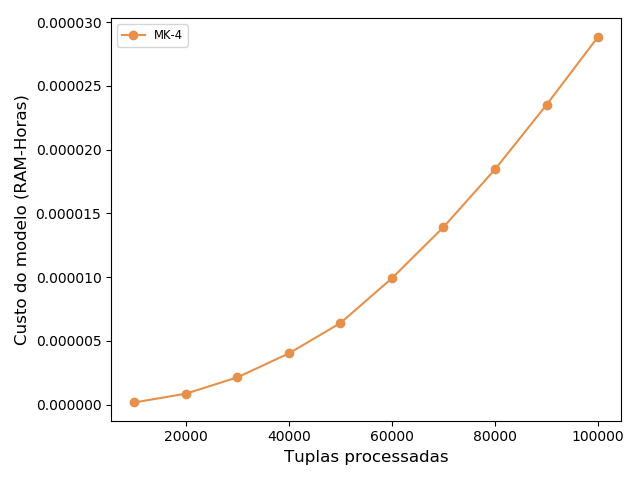
\includegraphics[width=\linewidth]{ram_incremental_drift_mk4.png}
\caption{Uso de memória para MK-4} \label{fig:incremental_1e}
\end{subfigure}
\end{minipage}

\caption[Gráficos de métricas no conjunto de dados  \textit{incremental\_drift}]{Gráficos de métricas no conjunto de dados  \textit{incremental\_drift}. Os gráficos de tempo de resposta e uso de memória precisaram ser separados para o método MK-4, devido aos altos valores.} \label{fig:incremental_drift}
\end{figure}



\begin{figure}[!htb]
\centering
\begin{subfigure}{0.485\textwidth}
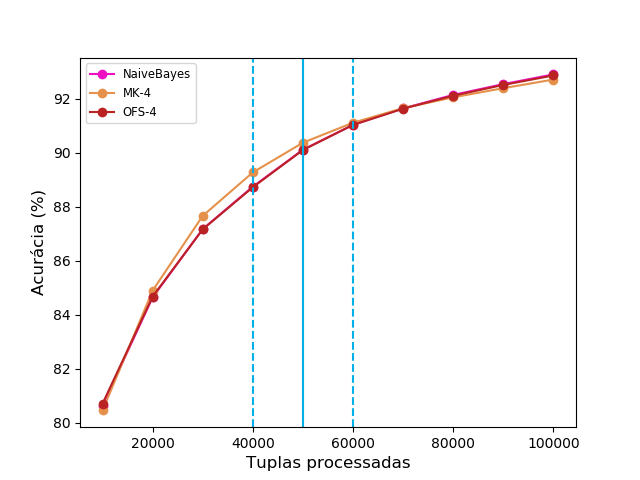
\includegraphics[width=\linewidth]{acc_gradual_drift.png}
\caption{Acurácia sequencial} \label{fig:gradual_1a}
\end{subfigure}
%\hspace*{\fill} % separation between the subfigures
\hfill
\begin{minipage}[b]{\textwidth} 
\begin{subfigure}[t]{0.485\textwidth}
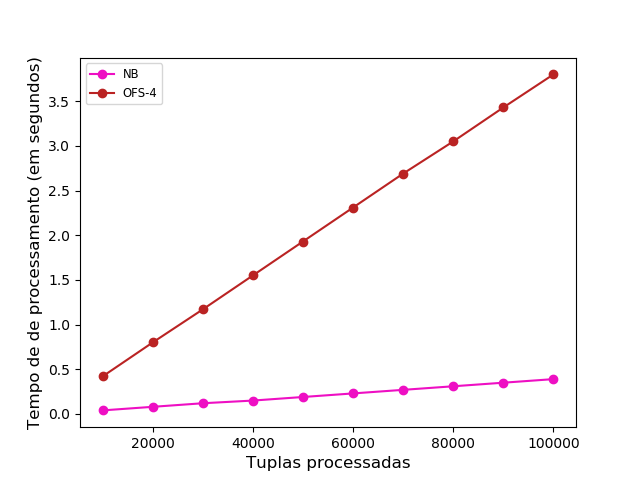
\includegraphics[width=\linewidth]{time_gradual_drift.png}
\caption{Tempo de resposta com Naïve Bayes e OFS-4} \label{fig:gradual_1b}
\end{subfigure}
%\hspace*{\fill} % separation between the subfigures
\hfill
\begin{subfigure}[t]{0.485\textwidth}
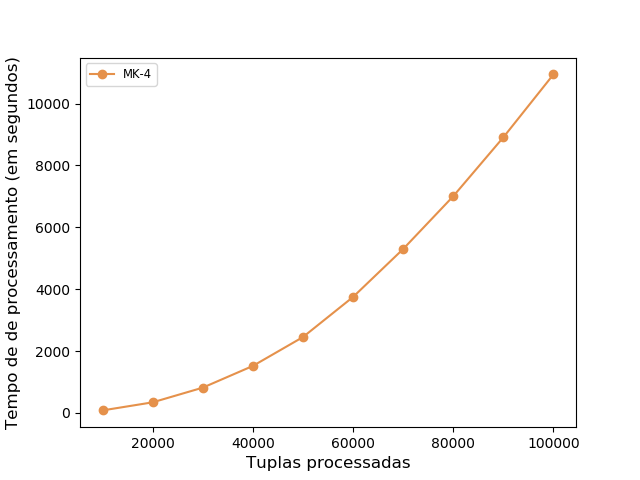
\includegraphics[width=\linewidth]{time_gradual_drift_mk4.png}
\caption{Tempo de resposta para MK-4} \label{fig:gradual_1c}
\end{subfigure}
\hfill
\begin{subfigure}[t]{0.485\textwidth}
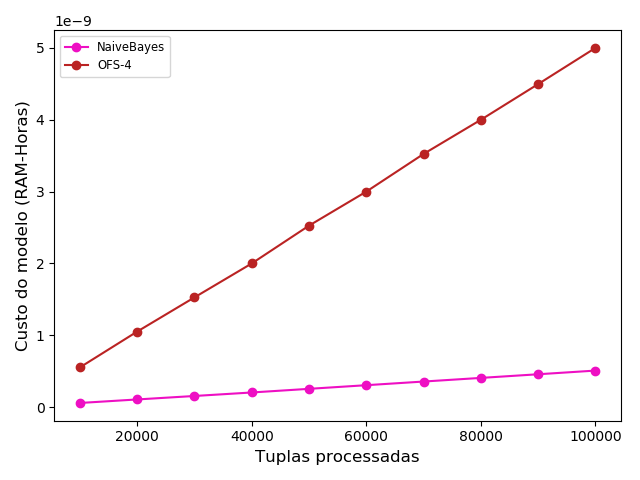
\includegraphics[width=\linewidth]{ram_gradual_drift.png}
\caption{Uso de memória com Naïve Bayes e OFS-4} \label{fig:gradual_1d}
\end{subfigure}
%\hspace*{\fill} % separation between the subfigures
\hfill
\begin{subfigure}[t]{0.485\textwidth}
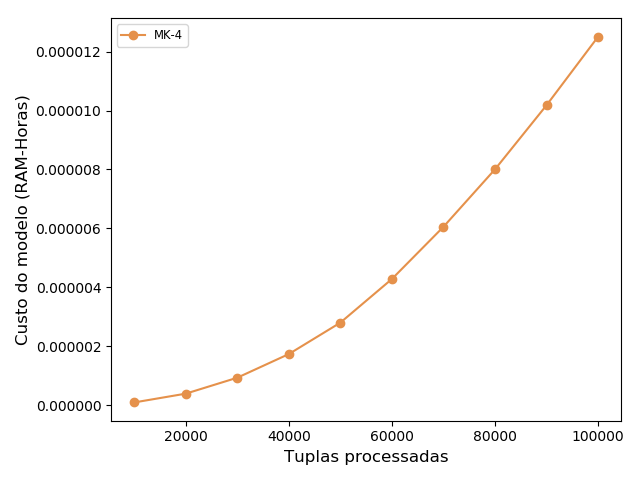
\includegraphics[width=\linewidth]{ram_gradual_drift_mk4.png}
\caption{Uso de memória para MK-4} \label{fig:gradual_1e}
\end{subfigure}
\end{minipage}

\caption[Gráficos de métricas no conjunto de dados \textit{gradual\_drift}]{Gráficos de métricas no conjunto de dados \textit{gradual\_drift}. As linhas pontilhadas e a reta em azul no gráfico de acurácia sequencial, representam, respectivamente, a janela de início/fim do \textit{drift} e o ponto exato de mudança. %Os gráficos de tempo de CPU e uso de memória precisaram ser separados para o método MK-4, devido aos altos valores.
} \label{fig:gradual_drift}
\end{figure}



\begin{figure}[!htb]
\centering
\begin{subfigure}{0.5\textwidth}
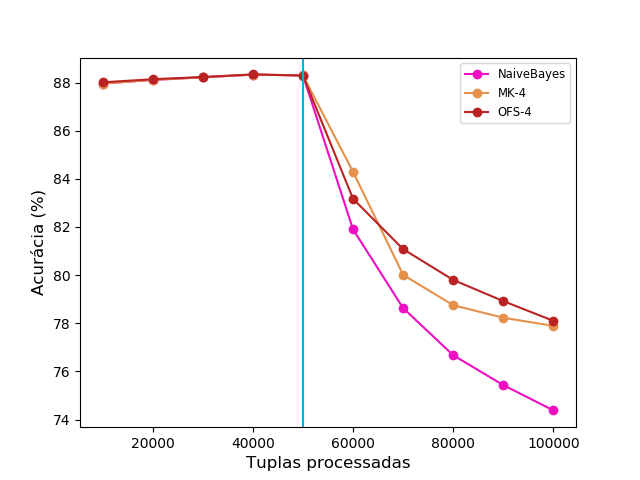
\includegraphics[width=\linewidth]{acc_sudden_drift.png}
\caption{Acurácia sequencial} \label{fig:sudden_1a}
\end{subfigure}
%\hspace*{\fill} % separation between the subfigures
\hfill
\begin{minipage}[b]{\textwidth} 
\begin{subfigure}[t]{0.485\textwidth}
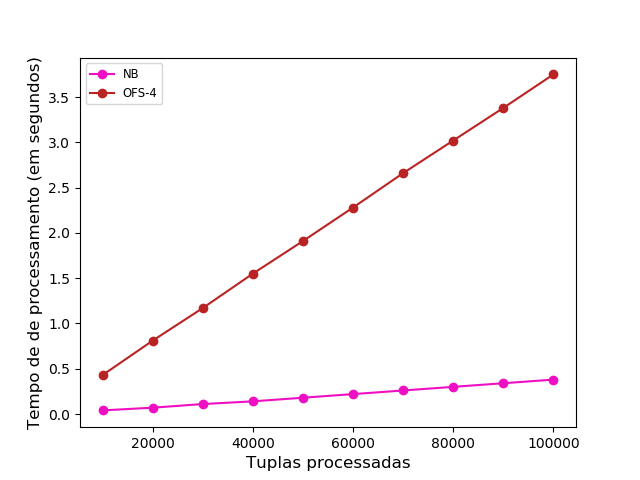
\includegraphics[width=\linewidth]{time_sudden_drift.png}
\caption{Tempo de resposta com Naïve Bayes e OFS-4} \label{fig:sudden_1b}
\end{subfigure}
%\hspace*{\fill} % separation between the subfigures
\hfill
\begin{subfigure}[t]{0.485\textwidth}
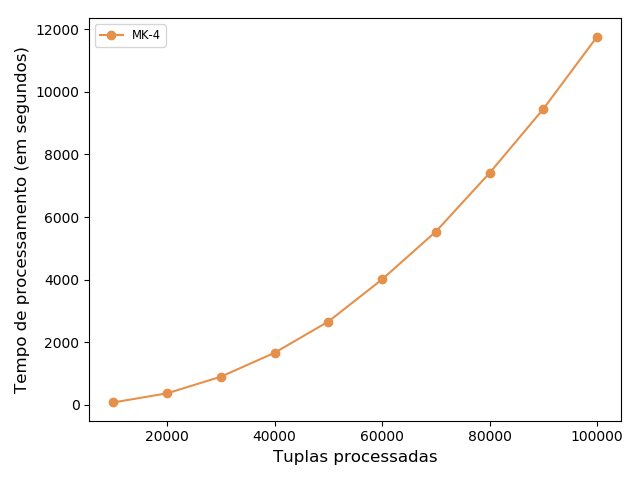
\includegraphics[width=\linewidth]{time_sudden_drift_mk4.png}
\caption{Tempo de resposta para MK-4} \label{fig:sudden_1c}
\end{subfigure}
\hfill
\begin{subfigure}[t]{0.485\textwidth}
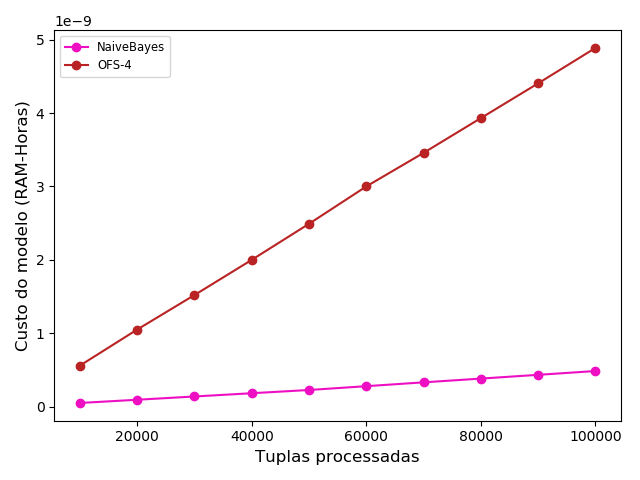
\includegraphics[width=\linewidth]{ram_sudden_drift.png}
\caption{Uso de memória com Naïve Bayes e OFS-4} \label{fig:sudden_1d}
\end{subfigure}
%\hspace*{\fill} % separation between the subfigures
\hfill
\begin{subfigure}[t]{0.485\textwidth}
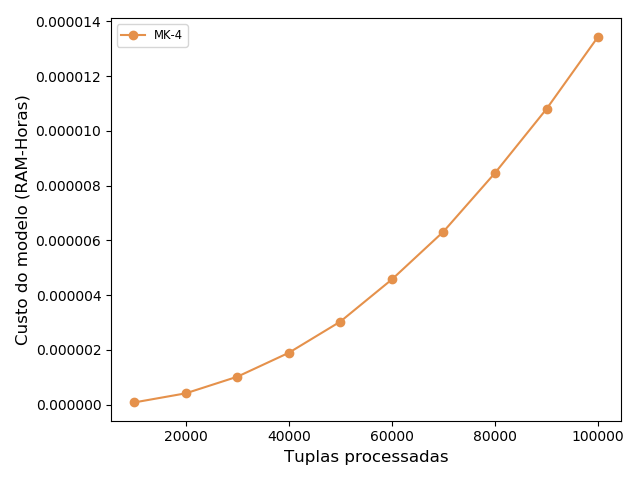
\includegraphics[width=\linewidth]{ram_sudden_drift_mk4.png}
\caption{Uso de memória para MK-4} \label{fig:sudden_1e}
\end{subfigure}
\end{minipage}

\caption[Gráficos de métricas no conjunto de dados \textit{sudden\_drift}]{Gráficos de métricas no conjunto de dados \textit{sudden\_drift}. A linha reta em azul no gráfico de acurácia sequencial representa o ponto exato de mudança. %Os gráficos de tempo de resposta e uso de memória precisaram ser separados para o método MK-4, devido aos altos valores.
} \label{fig:sudden_drift}
\end{figure}



\begin{figure}[!htb]
\centering
\begin{subfigure}{0.5\textwidth}
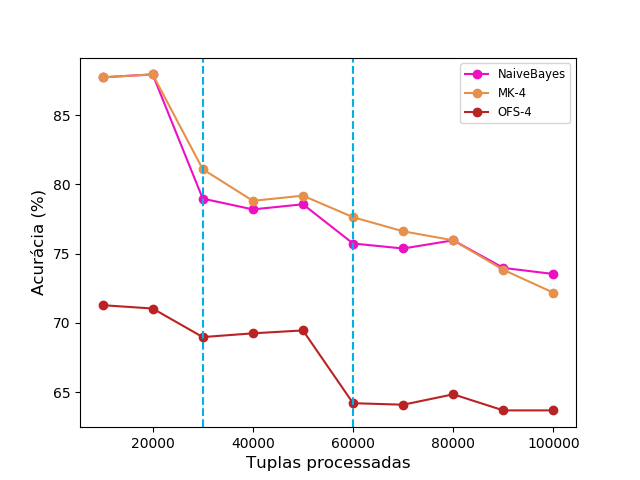
\includegraphics[width=\linewidth]{acc_recurrent_drift.png}
\caption{Acurácia sequencial} \label{fig:recurrent_1a}
\end{subfigure}
%\hspace*{\fill} % separation between the subfigures
\hfill
\begin{minipage}[b]{\textwidth} 
\begin{subfigure}[t]{0.485\textwidth}
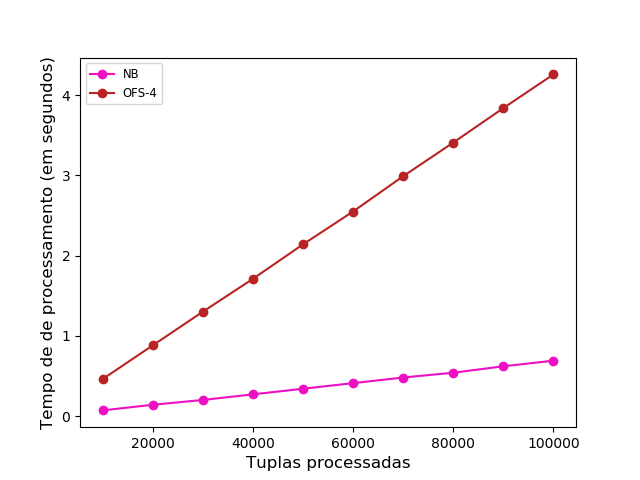
\includegraphics[width=\linewidth]{time_recurrent_drift.png}
\caption{Tempo de resposta com Naïve Bayes e OFS-4} \label{fig:recurrent_1b}
\end{subfigure}
%\hspace*{\fill} % separation between the subfigures
\hfil
\begin{subfigure}[t]{0.485\textwidth}
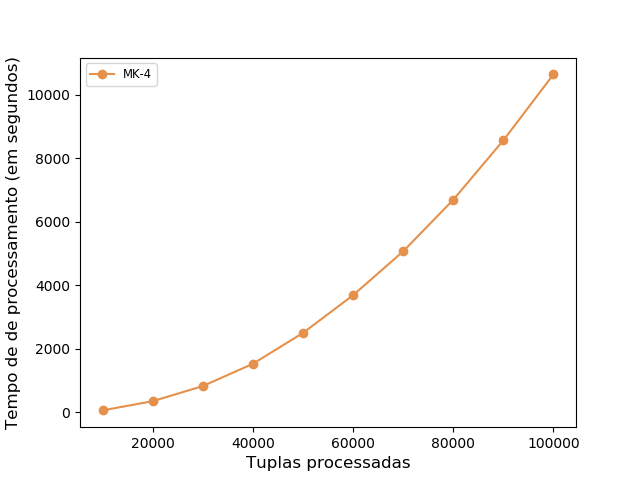
\includegraphics[width=\linewidth]{time_recurrent_drift_mk4.png}
\caption{Tempo de resposta para MK-4} \label{fig:recurrent_1c}
\end{subfigure}
\hfill
\begin{subfigure}[t]{0.485\textwidth}
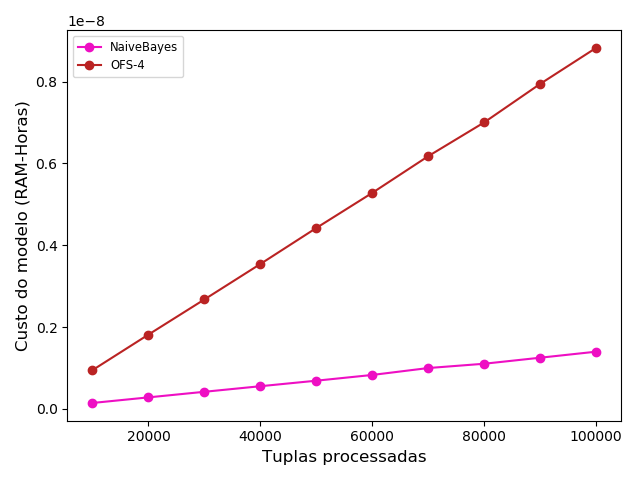
\includegraphics[width=\linewidth]{ram_recurrent_drift.png}
\caption{Uso de memória com Naïve Bayes e OFS-4} \label{fig:recurrent_1d}
\end{subfigure}
%\hspace*{\fill} % separation between the subfigures
\hfill
\begin{subfigure}[t]{0.485\textwidth}
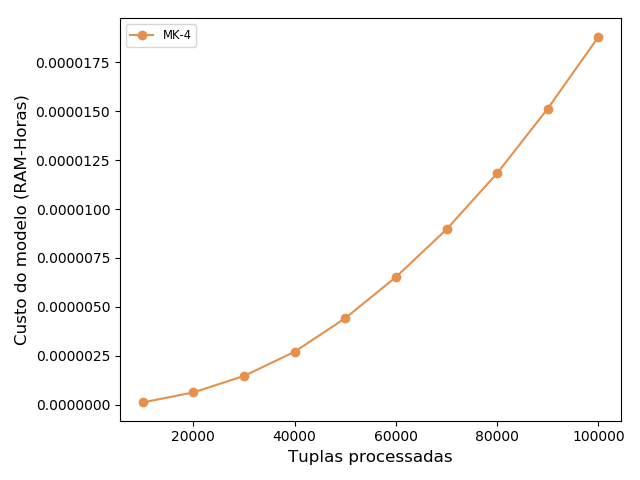
\includegraphics[width=\linewidth]{ram_recurrent_drift_mk4.png}
\caption{Uso de memória para MK-4} \label{fig:recurrent_1e}
\end{subfigure}
\end{minipage}

\caption[Gráficos de métricas no conjunto de dados \textit{recurrent\_drift}]{Gráficos de métricas no conjunto de dados \textit{recurrent\_drift}. As linhas pontilhadas no gráfico de acurácia sequencial representam respectivamente o início/fim da mudança. %Os gráficos de tempo de resposta e uso de memória precisaram ser separados para o método MK-4, devido aos altos valores.
} \label{fig:recurrent_drift}
\end{figure}

%[Andre] justei essa seção à anterior.
%\section{Discussões}\label{sec:res_discussoes}

\begin{figure}[!htb]
\centering
\begin{subfigure}[b]{0.485\textwidth}
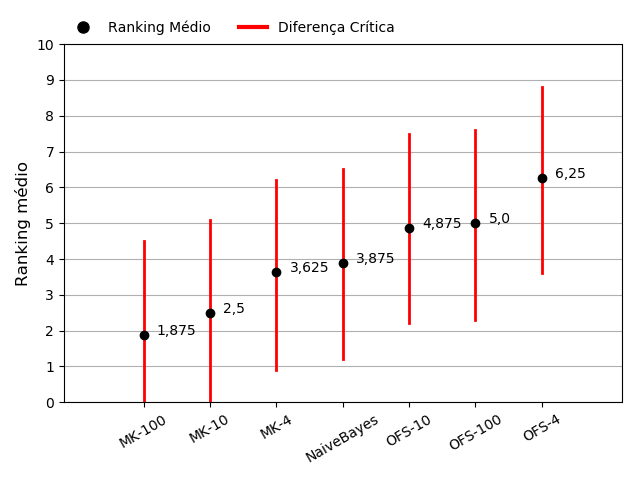
\includegraphics[width=\textwidth]{bonferroni_real.png}
\caption{Conjuntos de dados reais} \label{fig:bonferroni_1a}
\end{subfigure}
%\hspace*{\fill} % separation between the subfigures
\hfill %[Andre] Comentei a linha anterior
\begin{subfigure}[b]{0.485\textwidth}
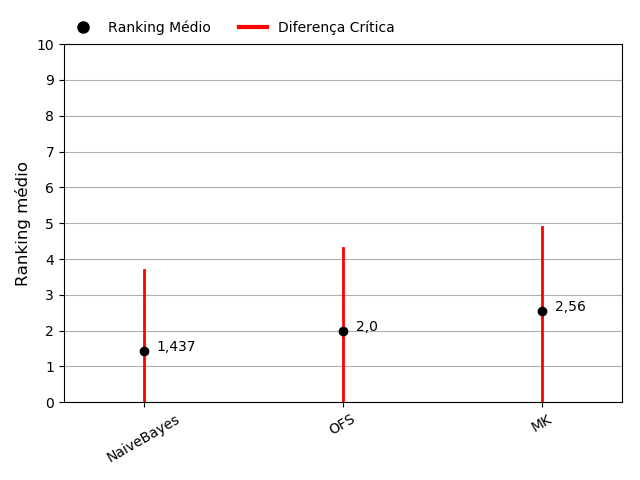
\includegraphics[width=\textwidth]{bonferroni_artificial.png}
\caption{Conjuntos de dados artificiais} \label{fig:bonferroni_1b}
\end{subfigure}
\caption{Gráficos de diferença crítica com o teste \textit{post-hoc} de Bonferroni-Dunn} \label{fig:bonferroni}
\end{figure}



Os resultados dos experimentos apontam  que o algoritmo MK apresentou os piores resultados em termos de tempo de resposta e quantidade de memória em todas as situações. Nos conjuntos de dados artificiais e com a janela de processamento tupla a tupla ($winSize=1$), chegou a consumir um tempo 500.000 vezes maior que os demais (7 horas contra aproximadamente 5 segundos para NB e OFS). Nas situações onde a janela de processamento foi maior,  o desempenho do MK foi relativamente superior aos obtidos pelo mesmo algoritmo. 

No conjunto \textit{incremental\_drift}, onde apresentou o pior resultado de todos em tupla a tupla, com $winSize=10$, o tempo de resposta foi reduzido em 700\%, atingindo cerca de 1 hora de processamento. Com $winSize=100$, passou para 5 minutos e, por fim, com $winSize=1000$, executou em 25 segundos. Neste último, a acurácia foi superior às outras janelas. Entretanto, ainda bem abaixo que a obtida com NB. O consumo de memória, consequentemente, também foi reduzido nessas proporções.

Quanto ao OFS, o mesmo possui velocidades competitivas ao NB. No pior cenário, com $winSize=1$ no conjunto de dados \textit{incremental\_drift}, analisou e classificou todas as tuplas em 5 segundos. Com $winSize=10,100 \text{ e } 1000$, precisou de, respectivamente, 
1,5 segundos, 0,9 segundos e 0,5 segundos.Neste último, ficou apenas 0,07 segundos atrás 
do algoritmo NB. Quanto ao consumo de memória, no pior dos cenários, o algoritmo OFS
precisou de $5\times10^{-9}$ RAM-horas e no melhor $5.2\times10^{-10}$ RAM-horas. Esse último valor é exatamente o mesmo obtido utilizando apenas o algoritmo NB.

Por fim, para validar os resultados de acurácia obtidos nos experimentos, foi utilizado o teste de Friedman, conforme indicado no Capítulo~\ref{chp:referencial}. Para um intervalo de confiança de $\alpha = 0,05$, o teste de Friedman indicou que a hipótese nula foi rejeitada. Diante disso, foi verificado se os resultados obtidos pelo NB foram significativamente superiores aos de MK e OFS utilizando o teste \textit{post-hoc} de Bonferroni-Dunn. A Figura~\ref{fig:bonferroni}, na página \pageref{fig:bonferroni}, apresenta os resultados para ambos os conjuntos de dados reais e artificiais, considerando todas as janelas de processamento.

Para os conjuntos reais e artificiais, em um intervalo de confiança de $\alpha=0,05$, a diferença crítica foi $2,638$ e $2,343$, respectivamente. Analisando os resultados, há evidências de que, embora o NB obtenha acurácias finais superiores na maioria dos cenários (4 de 6), essa superioridade não é significativa, pois considerando bases de dados reais e artificiais seus resultados são estatisticamente equivalentes aos de MK e OFS. Esses resultados estão abaixo da diferença crítica em todos os cenários avaliados. 

\citeonline{Katakis2005} apresentam em seu artigo os resultados da acurácia de seu método utilizando o conjunto de dados \textit{spam\_data}. Esses resultados são similares aos obtidos nos experimentos aqui apresentados. Entretanto, os autores não avaliam nenhuma outra métrica. Desse modo, os experimentos deste trabalho demonstram que, embora a acurácia final seja de fato razoável, o consumo de memória e tempo de resposta elevados inviabilizam a utilização deste método. 

Entretanto, analisando as acurácias sequenciais desse algoritmo, o mesmo apresenta a melhor adaptabilidade a mudanças de conceitos graduais e súbitas quando a dimensionalidade dos fluxos é alta e justifica a utilização de seleção de atributos, e nos casos de mudanças recorrentes, mesmo em baixa dimensionalidade. Esse fato demonstra que há potencial na utilização deste método em cenários de mudanças de conceito, em especial em cenários de alta dimensionalidade, caso o tempo de resposta e o consumo de memória RAM sejam reduzidos.

Uma possível solução para esse cenário é a utilização da Computação de Alto Desempenho para a utilização de bibliotecas que permitam que os trechos de código mais custosos computacionalmente sejam paralelizados. Outra alternativa é a utilização de Unidades de Processamento Gráfico (\textit{Graphics Processing Units -- GPU}) para realização do cálculo de avaliação dos atributos. Desta forma, o processador ficaria responsável apenas pela classificação dos dados, o que diminuiria a carga de trabalho e concorrência, reduzindo o tempo necessário para avaliação dos atributos e consequentemente da classificação final.

Em seu artigo, \citeonline{Wang2014} apresentam os resultados de uma avaliação sistemática do desempenho do OFS em diferentes situações, em especial com conjuntos de dados em larga escala. Nesses cenários, o algoritmo OFS demonstra uma alta capacidade para lidar com grandes volumes de dados, tanto no número de tuplas quanto na quantidade de atributos, em situações onde não há variação probabilística dos dados. 

Contudo, os experimentos realizados neste trabalho apontam que o algoritmo OFS é sensível à mudanças de conceitos, apresentando acurácia inferior ao algoritmo NB em cinco dos seis cenários avaliados. Além disso, também obteve uma acurácia inferior ao MK em conjuntos de dados com alta dimensionalidade, o que pode torná-lo inviável nessas situações. Avaliando a acurácia sequencial, o OFS mostrou a maior adaptabilidade à mudanças súbitas quando a dimensão dos dados é baixa. 

Desse modo, as evidências apontam que, no geral,  a utilização de um método de classificação supervisionada sem a seleção de atributos apresenta resultados superiores quando comparados a utilização do Método de Katakis com Ganho de Informação e o algoritmo \textit{OnlineFeatureSelection} em fluxos de dados com mudanças de conceito. Entretanto, por apresentar uma maior adaptabilidade às mudanças de conceito no quesito capacidade preditiva em três dos seis cenários, o Método de Katakis com Ganho de Informação possui um potencial de utilização caso seus problemas de desempenho sejam solucionados.


\section{Considerações finais deste capítulo}\label{sec:res_consideracoes} 

Este capítulo apresentou os resultados dos experimentos realizados com os algoritmos MK e OFS. O algoritmo MK apresentou os piores tempos de resposta e consumo de memória, mas acurácias aproximadas da classificação sem seleção de atributos (apenas com NB), superando-o em uma situação e superior ao OFS em quatro dos seis cenários. 

Já o algoritmo OFS demonstrou tempos de resposta e consumo de memória relativamente próximos aos obtidos com o algoritmo NB. Em termos de acurácia, o algoritmo OFS mostrou maior adaptabilidade às mudanças súbitas em fluxos com uma baixa dimensionalidade, superando os demais algoritmos considerados nesse cenário. Contudo, esse algoritmo obteve resultados inferiores em conjuntos com alta dimensionalidade.

A hipótese nula de semelhança dos algoritmos foi rejeitada com o teste de Friedman, e o teste \textit{post-hoc} de Bonferroni-Dunn apresentou evidências de equivalência estatística das acurácias de NB em comparação com MK e OFS em todos os cenários. 